\documentclass[letterpaper]{article} %DO NOT CHANGE THIS
\usepackage{aaai19}  %Required
\usepackage{times}  %Required
\usepackage{helvet}  %Required
\usepackage{courier}  %Required
\usepackage{url}  %Required
\usepackage{graphicx}  %Required

\usepackage{amsmath,amsfonts,amssymb}
\usepackage{paralist}
\usepackage{color,xcolor}
\usepackage{bm}
\usepackage{multirow}
\usepackage{makecell}
\usepackage{caption}
\usepackage[linesnumbered,lined]{algorithm2e}
\usepackage{todonotes}

\frenchspacing  %Required
\setlength{\pdfpagewidth}{8.5in}  %Required
\setlength{\pdfpageheight}{11in}  %Required

%PDF Info Is Required:
%\pdfinfo{
%	/Title (Disentangled Representation Learning for Text Style Transfer)
%	/Author (Vineet John, Lili Mou, Hareesh Bahuleyan, Olga Vechtomova)
%}


% bold x for equations
\newcommand{\rmx}{\mathrm x} 
% used for table headers
\newcommand{\tabh}[1]{\multicolumn{1}{c|}{\textbf{#1}}}  
% used for the top left cell in a table
\newcommand{\tabc}[2]{\multicolumn{1}{|c||}{\multirow{#1}{*}{\textbf{#2}}}} 
% used for denoting the loss symbol with a subscript
\newcommand{\loss}[1]{J_{\text{#1}}}
% used for denoting the lambda symbol with a subscript
\newcommand{\hyp}[1]{\lambda_{\text{#1}}}
% used for denoting the theta symbol with a subscript
\newcommand{\nnweight}[1]{\bm{\theta_{\text{#1}}}}
% used for denoting the weight symbol (w) with a subscript
\newcommand{\weight}[1]{\bm{w_{\text{#1}}}}
% used for denoting the bias symbol (b) with a subscript
\newcommand{\bias}[1]{b_{\text{#1}}}
% custom author-year citation
\newcommand{\citeay}[1]{\citeauthor{#1} \shortcite{#1}}

\title{Disentangled Representation Learning for Non-Parallel Text Style Transfer}

%\author{
%	Vineet John \\
%	University of Waterloo \\
%	{\tt vineet.john@uwaterloo.ca} \\
%	\And
%	Lili Mou \\
%	AdeptMind Research \\
%	{\tt doublepower.mou@gmail.com}\\{\tt lili@adeptmind.ai} \\
%	\AND
%	Hareesh Bahuleyan \\
%	University of Waterloo \\
%	{\tt hpallika@uwaterloo.ca} \\
%	\And
%	Olga Vechtomova \\
%	University of Waterloo \\
%	{\tt ovechtom@uwaterloo.ca} \\
%}

\date{}
\begin{document}
\maketitle
\graphicspath{{images/}}

\begin{abstract}
	This paper tackles the problem of disentangling the latent variables of style and content in language models.
	We propose a simple yet effective approach, which incorporates auxiliary multi-task and adversarial objectives for label prediction and bag-of-words prediction, respectively.
	We show, both qualitatively and quantitatively, that the style and content are indeed disentangled in the latent space.
	This disentangled latent representation learning method is applied to attribute (e.g. style) transfer on non-parallel corpora.
	We achieve similar content preservation scores compared to previous state-of-the-art approaches, and significantly better style-transfer strength scores.
	\footnote{Our code and data are publicly available at \url{https://bit.ly/2wxps69} (The materials are properly anonymized during double-blind review.)}
	% \footnote{\url{https://github.com/vineetjohn/linguistic-style-transfer}}.
\end{abstract}

% 


\section{Introduction}

The neural network has been a successful learning machine during the past decade due to its highly expressive modeling capability, which is a consequence of multiple layers of non-linear transformations of input features.
Such transformations, however, make intermediate features ``latent,'' in that they do not have explicit meanings and are not explainable.
Therefore, neural networks are usually treated as black-box machinery.

Disentangling the latent space of neural networks has become an increasingly important research topic.
In the image domain, for example, \citeay{chen2016infogan} use adversarial and information maximization objectives to produce interpretable latent representations that can be tweaked to adjust writing style for handwritten digits, as well as lighting and orientation for face models.
\citeay{mathieu2016disentangling} utilize a convolutional autoencoder to achieve the same objective.
However, this problem is not well explored in natural language processing.

In this paper, we address the problem of disentangling the latent space of neural networks for text generation.
Our model is built on an autoencoder that encodes a sentence to the latent space (vector representation) by learning to reconstruct the sentence itself.
We would like the latent space to be disentangled with respect to different features, namely, \textit{style} and \textit{content} in our task.

To accomplish this, we propose a simple yet effective approach that combines multi-task and adversarial objectives. We artificially divide the latent representation into two parts: the style space and content space. In this work, we consider the sentiment of a sentence as the style.
We design auxiliary losses, enforcing our model to separate style and content latent spaces.
In particular, the multi-task loss operates on a latent space to ensure that the space does contain the information we wish to encode.
The adversarial loss, on the contrary, minimizes the predictability of information that should not be contained in that space.
In previous work, researchers typically work with the style, or specifically, sentiment space~\cite{hu2017toward,shen2017style,fu2017style,zhao2018adversarially}, but simply ignore the content space, as it is hard to formalize what ``content'' actually refers to.

In our paper, we propose to approximate the content information by bag-of-words (BoW) features, where we focus on style-neutral, non-stop words.
Along with traditional style-oriented auxiliary losses, our BoW multi-task loss and BoW adversarial loss make the style and content spaces much more disentangled from each other.

The disentangled latent space can be directly used for text style-transfer~\cite{hu2017toward,shen2017style,fu2017style}, where a model shall be able to generate a sentence with the same content but a different style.
Since it is difficult to obtain sentence pairs with the same content and differing styles, we follow the setting where we train our model on a non-parallel but style-labeled corpora. We call this \textit{non-parallel text style transfer}.
To accomplish this, we train an autoencoder with disentangled latent space during training.
For style-transfer inference, we simply use the autoencoder to encode the content vector of a sentence, but ignore its encoded style vector.
We then infer from the training data an empirical embedding of the style that we would like to transfer to.
The encoded content vector and the inferred style vector are concatenated and fed to the decoder.
Such grafting technique enables us to obtain a new sentence similar in content to the input sentence, but with a different style.

We conducted experiments on two benchmark datasets of customer reviewers.
Both qualitative and quantitative results show that the style vector and the content vector are indeed disentangled well.
In the style-transfer evaluation, we achieve significantly better style-transfer strength compared with previous results, while obtaining better or comparable content preservation scores.
Ablation tests also show that the auxiliary losses can be combined well, each playing its own role in disentangling the latent space.


\section{Related Work}

Disentangling neural networks' latent space has been explored in the image processing domain in the recent years, and researchers have successfully disentangled rotation features, color features, etc.~\cite{chen2016infogan,luan2017deep}.
Some image characteristics (e.g., artistic style) can be captured well by certain statistics \cite{gatys2016image}.
In other work, researchers adopt data augmentation techniques to learn a disentangled latent space~\cite{kulkarni2015deep,champandard2016semantic}.

In natural language processing, the definition of ``style'' itself is vague, and as a convenient starting point, NLP researchers often treat sentiment as a salient style of text.
\citeay{hu2017toward} manage to control the sentiment by using discriminators to reconstruct sentiment and content from generated sentences.
However, there is no evidence that the latent space would be disentangled by this reconstruction.
\citeay{shen2017style} use a pair of adversarial discriminators to align the recurrent hidden decoder states of original and style-transferred sentences, for a given style.
\citeay{fu2017style} propose two approaches: using a style embedding matrix, and using style-specific decoders for style-transfer.
They apply an adversarial loss on the encoded space to discourage encoding style in the latent space of an autoencoding model. However, all the above approaches only deal with the style information and simply ignore the content part.

\citeay{zhao2018adversarially} extend the multi-decoder approach and use a Wasserstein-distance penalty to align content representations of sentences with different styles. However, the Wasserstein penalty is applied to  empirical samples from the data distribution, and is much indirect than our BoW-based auxiliary losses.

Recently, \citeay{rao2018dear} treat the formality of writing as a style, and create a parallel corpus for style transfer with sequence-to-sequence models. This is beyond the scope of our paper, as we focus on non-parallel text style transfer.

Our paper differs from the previous work in that both our style space and content space are encoded from the input. We apply several auxiliary losses to ensure that each space encodes and only encodes the desired information. Such disentanglement of latent space has its own research interest in the deep learning community.
The disentangled representation can then be directly applied to non-parallel text style-transfer tasks, as in the aforementioned studies.


\section{Approach}

In this section, we describe our approach in detail, shown in Figure~\ref{fig:overview}.
Our model is built upon an autoencoder with a sequence-to-sequence neural network~\cite{sutskever2014sequence}.
Then, we introduce the multi-task and adversarial auxiliary losses for both style and content space.
Finally, we present our approach to style transfer in the context of natural language generation.

\begin{figure}[!t]
	\centering
	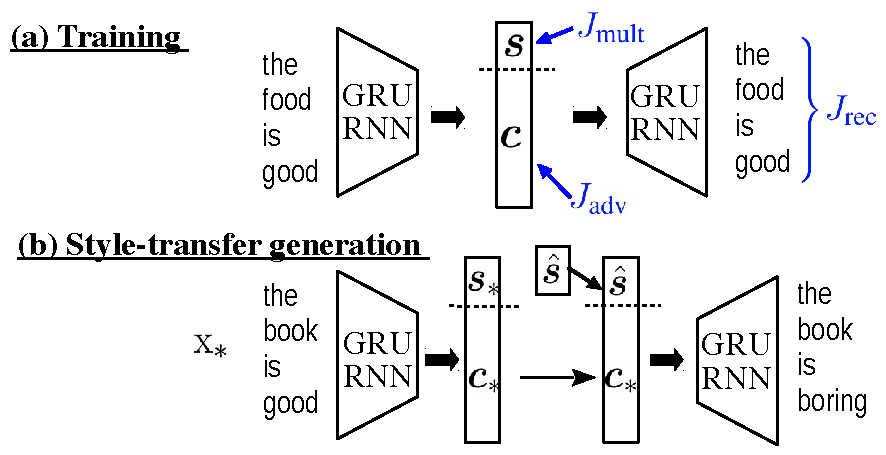
\includegraphics[width=.9\linewidth]{model-overview}
	\caption{Overview of our approach.}
	\label{fig:overview}
\end{figure}

\subsection{Autoencoder} \label{ssec:seq2seq-autoencoder}

An autoencoder encodes an input to a latent vector space, from which it decodes the input itself. The latent vector space is usually of much smaller dimensionality than input data, and the autoencoder learns salient and compact representations of data during the reconstruction process.
This serves as our primary learning objective.
Besides, we also use the autoencoder for text generation in the style-transfer application.

Let $\rmx=(x_1, x_2, \cdots x_n)$ be an input sequence with $n$ tokens.
The encoder recurrent neural network (RNN) with gated recurrent units (GRU) \cite{cho2014learning} encodes $\rm x$ and obtains a hidden state $\bm h$.
Then a decoder RNN generates a sentence, which ideally should be $\rmx$ itself.
Suppose at a time step $t$, the decoder RNN predicts the word $x_t$ with probability $p(x_t|\bm h, x_1\cdots x_{t-1})$. Then the autoencoder is trained with a sequence-aggregated cross-entropy loss, given by
\begin{equation}
	\loss{AE}(\nnweight{E},\nnweight{D})= -\sum_{t=1}^n \log p(x_t|\bm h, x_1\cdots x_{t-1})
\end{equation}
where $\nnweight{E}$ and $\nnweight{D}$ are the parameters of the encoder and decoder, respectively.\footnote{For brevity, we only present the loss for a particular data point (i.e., a sentence) throughout out paper. The total loss sums over all data points, but is implemented with mini-batches.} Both the encoder and decoder are deterministic functions in the original autoencoder model~\cite{}, and thus we call it a \textit{deterministic autoencoder} (DAE).

\subsubsection{Variational Autoencoder.}

In addition to the deterministic auto-encoding objective presented above, we also tried a variational autoencoder (VAE) \cite{kingma2013auto}, which imposes a probabilistic distribution to the latent vector. The Kullback-Leibler (KL) divergence \cite{kullback1951information} penalty is added to the loss function to regularize the latent space. The decoder reconstructs data based on the sampled latent vector from its posterior distribution.

Formally, the autoencoding loss in the variational version is
\begin{equation}
	\loss{AE}(\nnweight{E}, \nnweight{D}) =
	- \mathbb{E}_{q_{E}(\bm h|\rmx)} [\log p(\rmx|\bm h)]
	+ \hyp{kl}\operatorname{KL}(q_{E}(\bm h|\rmx)\|p(\bm h))
\end{equation}
where $\hyp{kl}$ is the hyperparameter balancing the reconstruction loss and the KL terms. $p(\bm h)$ is the prior, set to the standard normal distribution $\mathcal{N}(\bm 0,\mathrm I)$.

The motivation for using VAE as opposed to DAE is  that the reconstruction is based on the samples of the posterior, which theoretically populates to the neighborhood and thus smooths the latent space. \citeay{bowman2016generating} show that VAE generates more fluent sentences than DAE.

Besides the above autoencoding loss, we design several auxiliary losses to disentangle the latent space. In particular, we hope that $\bm h$ can be separated into two spaces $\bm s$ and $\bm c$, representing style and content respectively, i.e., $\bm h = [\bm s ; \bm c]$, where $[\cdot;\cdot]$ denotes concatenation.
This is accomplished by the auxiliary losses described in the rest of this section.


\subsection{Style-Oriented Losses}

We first design auxiliary losses that ensures the style information is contained in the style space $\bm s$. This involves a multi-task losses that ensures $\bm s$ is discriminative for the style, as well as an adversarial loss that ensures $\bm c$ is not discriminative for the style.

\subsubsection{Multi-Task Loss for Style.} \label{ssec:multitask-style-objective}
Although the corpus we use is non-parallel, we assume that each sentence is labeled with its style. In particular, we treat the sentiment as the style of interest, following most previous work~\cite{hu2017toward,shen2017style,fu2017style}, and each sentence is labeled with a binary sentiment tag (positive or negative).

We build a classifier on the style space that predicts the style label. Formally, a logistic regression layer is applied to the style vector $\bm s$, given by
\begin{equation} \label{eqn:class-pred}
	y = \sigma({\weight{mul(s)}}^\top \bm s + \bias{mul(s)})
\end{equation}
where $\sigma$ is the sigmoid function, and $\nnweight{mul(s)}=[\weight{mul(s)}; \bias{mul(s)}]$ are parameters for multi-task learning of style, and $y$ is the output of the logistic unit.

The classifier is trained with a simple cross-entropy loss. For binary classification as in out scenario, it takes the form
\begin{equation} \label{eqn:style-multi-task-loss}
	\loss{mul(s)}(\nnweight{E};\nnweight{mul(s)}) =
	- t \log y - (1-t)\log (1-y)
\end{equation}
where $\nnweight{E}$ are the encoder's parameters, and $t$ is the groundtruth target label.


We train the style classifier at the same time as the autoencoding loss. Thus, this could be viewed as \textit{multi-task} learning, incentivizing the entire model to not only decode the sentence, but also predict its sentiment from the style vector $\bm  s$. We denote it by ``mul(s).''
Similar multi-task losses are used in previous work for sequence-to-sequence learning \cite{luong2015multi}, sentence representation learning \cite{jernite2017discourse} and sentiment analysis \cite{balikas2017multitask}, among others.


\subsubsection{Adversarial Loss for Style.}
\label{ssec:adversarial-style-objective}

The multi-task loss could only ensure the style space does contain style information. However, it does not say

We apply an adversarial loss to disentangle the content space from style information.

The idea of adversarial loss is to introduce an objective that deliberately discriminates the true style label using the content vector $\bm c$.
Then the autoencoder is trained to learn a content vector space that its adversary cannot predict style information from.

Concretely, the adversarial discriminator predicts style by computing a softmax distribution over the possible class labels
\begin{equation}
	y = \sigma({\weight{dis(s)}}^\top \bm c + \bias{dis(s)})
\end{equation}
where $\nnweight{dis(s)}=[\weight{dis(s)}; \bias{dis(s)}]$ are the parameters of the adversary, and $y$ is the predicted label distribution.

It is trained by minimizing the following objective, using a cross-entropy loss.
\begin{equation} \label{eqn:adv-disc-loss}
	\loss{dis(s)} (\nnweight{dis(s)}) =
	- \mathbb{E} [\log p(y' | \bm c; \nnweight{dis(s)})]
\end{equation}
where $y'$ is the true label distribution.

The adversarial loss appears similar to the multi-task loss as in Equation \ref{eqn:style-multi-task-loss}.
However, it should be emphasized that, for the adversary, the gradients are not propagated back to the autoencoder, i.e. the variables in $\bm c$ are treated as shallow features.

Having trained an adversary, we would like the autoencoder to be tuned in such an \textit{ad hoc} fashion, that $\bm c$ is not discriminative in style.
In other words, we penalize the Shannon entropy of the adversary's prediction, given by
\begin{equation}
	\loss{adv(s)}(\nnweight{E})=\mathcal{H}(y|\bm c; \nnweight{dis(s)})
\end{equation}
where $\mathcal{H}(p)=-\sum_{i\in\text{labels}}p_i\log p_i$ is the entropy and $y$ is the predicted distribution over the style labels.
The adversarial objective is maximized, in this phase, with respect to the encoder.
This objective helps the autoencoder maximize the uncertainty of the discriminator's predicted probability distribution, which occurs when the distribution is uniform.

\subsection{Content-Oriented Losses}

\subsubsection{Content Classifier} \label{ssec:multitask-content-objective}

In a similar vein to the multi-task style prediction objective, we also try to predict the content, represented by a bag-of-words (BoW), from the content vector $\bm c$.
Here, we define the content of the sentence as the words from the original sentence without any words that are discriminative of style.

The input sentences $\rmx$ are represented as vectors of the same size as the corpus vocabulary, with each index of the vector denoting the frequency of a word's presence in the sentence.
For a sentence $s$ with $N$ tokens, a word $w_*$'s BoW probability is given by $\frac{\sum_{i=1}^{N}{(1 | w_i = w_*)}}{N}$.
We exclude stopwords and sentiment words \cite{hu2004mining} from the BoW representation.

We introduce a multi-label classifier over the BoW vocabulary
\begin{equation} \label{eqn:bow-pred}
	v = \sigma({\weight{mul(c)}}^\top \bm s + \bias{mul(c)})
\end{equation}
where $\nnweight{mul(c)}=[\weight{mul(c)}; \bias{mul(c)}]$ are the classifier's parameters for multi-task learning, and $v$ is the predicted BoW distribution.

This is trained using a simple cross-entropy loss
\begin{equation} \label{eqn:content-multi-task-loss}
	\loss{mul(c)}(\nnweight{E};\nnweight{mul(c)}) =
	- \mathbb{E} [\log p(v' | \bm s; \nnweight{mul(c)})]
\end{equation}
where $\nnweight{E}$ are the encoder's parameters, and $v'$ is the true BoW distribution.


\subsection{Adversarial Discriminators}

The above multi-task losses, although essential for improving the style and content predictability from the separate spaces, does not guarantee that the style is not present in the content space and vice-versa. For this purpose, we use adversarial training objectives, inspired by adversarial generation~\cite{goodfellow2014generative}, adversarial domain adaptation~\cite{liu2017adversarial}, and adversarial style-transfer~\cite{shen2017style,fu2017style}.



\subsubsection{Content Discriminator} \label{ssec:adversarial-content-objective}

We also propose a bag-of-words (BoW) discriminator on the style space to make our approach complete.
The motivation is to emulate the adversarial signal provided by the style discriminator, and do the same for the content.

The BoW discriminator uses the style vector $\bm s$ produced by the autoencoder model, and tries to predict the true BoW distribution using a set of parameters that are distinct from those of the autoencoder.
The discriminator uses a softmax activation to predict the occurrence frequency of each word in the original sentence, between $0$ and $1$.
\begin{equation}
	v = \sigma({\weight{dis(c)}}^\top \bm s + \bias{dis(c)})
\end{equation}
where $\nnweight{dis(c)}=[\weight{dis(c)}; \bias{dis(c)}]$ are the classifier's parameters for BoW prediction, and $v$ is the predicted BoW distribution.

This objective is trained in a similar method to the style adversary, using a cross-entropy loss
\begin{equation} \label{eqn:adv-bow-disc-loss}
	\loss{dis(c)}(\nnweight{dis(c)}) =
	- \mathbb{E} [\log p(v' | \bm s; \nnweight{dis(c)})]
\end{equation}
where $v'$ is the true BoW distribution.

We also refrain from propagating the effects of this discriminator loss $\loss{dis(c)}$ to the encoder parameters, ensuring that the parameters that each adversary and the autoencoder can update are mutually exclusive.

Similar to the style adversary, the empirical Shannon entropy of the predicted distribution is provided as a training signal for the autoencoder model to maximize.
\begin{equation}
	\loss{adv(c)}(\nnweight{E}) = \mathcal{H}(v | \bm s; \nnweight{dis(c)})
\end{equation}
where $v$ is the predicted word distribution.

The motivation for this adversarial loss is similar to the one used in the context of the style discriminator.
We want to encourage the encoder to learn a representation of style $\bm s$ that the BoW discriminator cannot predict most of the original words from.

\subsection{Training Process}

The overall loss $\loss{ovr}$, used for the autoencoder, is thus comprised of four distinct objectives: the reconstruction objective, the multi-task objectives, and the adversarial objectives for style and content.
\begin{align}
	\loss{ovr} = & \loss{AE}(\nnweight{E}, \nnweight{D})  \nonumber                                                                   \\
	             & + \hyp{mul(s)} \loss{mul(s)} (\nnweight{E},\nnweight{mul(s)}) - \hyp{adv(s)} \loss{adv(s)}(\nnweight{E}) \nonumber \\
	             & + \hyp{mul(c)} \loss{mul(c)} (\nnweight{E},\nnweight{mul(c)}) - \hyp{adv(c)} \loss{adv(c)}(\nnweight{E})
\end{align}
where $\hyp{mul(s)}$, $\hyp{adv(s)}$ and $\hyp{adv(c)}$ balance the model's auxiliary losses.

To put it all together, the model training consists of a loop involving the processes shown in Algorithm \ref{alg:training-process}.
\begin{algorithm}[ht]
	\While{epochs remaining}{
		minimize $\loss{dis(s)}(\nnweight{dis(s)})$ w.r.t. $\nnweight{dis(s)}$\;
		minimize $\loss{dis(c)}(\nnweight{dis(c)})$ w.r.t. $\nnweight{dis(c)}$\;
		minimize $\loss{ovr}$ w.r.t. $\nnweight{E}, \nnweight{D}, \nnweight{mul(s)}, \nnweight{mul(c)}$\;
	}
	\caption{Training process.}
	\label{alg:training-process}
\end{algorithm}

We use the Adam optimizer \cite{kingma2014adam} for the autoencoder and the RMSProp optimizer \cite{tieleman2012lecture} for the discriminators, each with an initial learning rate of $10^{-3}$, and train the model for 20 epochs.
The word embedding layer is initialized using pre-trained Word2Vec embeddings \cite{mikolov2013distributed} from the training set.
Both the autoencoder and the discriminators are trained once per epoch with $\hyp{mul(s)} = 10$, $\hyp{mul(c)} = 3$, $\hyp{adv(s)} = 1$ and $\hyp{adv(c)} = 0.03$.
These hyperparameters were identified by performing a log-scale grid search within 2 orders of magnitude, and choosing the hyperparameters that yielded the best results.
The recurrent unit size is $256$, the style vector size is $8$, and the content vector size is $128$.
We append the latent vector $\bm h$ to the hidden state at every time step of the decoder \cite{bahuleyan2017variational}.
For the VAE model, we enforce the KL-divergence penalty on both the style and content posterior distributions, using $\hyp{kl(s)}$ and $\hyp{kl(c)}$, respectively.
We set $\hyp{kl(s)} = 0.03$ and $\hyp{kl(c)} = 0.03$ and use the $\operatorname{sigmoid}$ KL-weight annealing schedule proposed by \citeay{bahuleyan2018probabilistic}.


\subsection{Generating Style-Transferred Sentences} \label{ssec:sentence-generation}

A direct application of our disentangled latent space is style-transfer for natural language generation.
For example, we can generate a sentence with generally the same meaning (content) but a different style (e.g. sentiment).

Let $\rmx^*$ be an input sentence with $\bm s^*$ and $\bm c^*$ being the encoded, disentangled style and content vectors, respectively.
If we would like to transfer its content to a different style, we compute an empirical estimate of the target style's vector $\hat{\bm s}$ by
\begin{equation*}
	\hat{\bm s}=\frac{\sum_{i\in\text{target style}}\bm s_i}{\text{\# target style samples}}
\end{equation*}
The inferred target style $\hat{\bm s}$ is concatenated with the encoded content $\bm c^*$ for decoding style-transferred sentences (Figure~\ref{fig:overview}).


\section{Experiments}

\begin{table*}[ht]
	\centering
	\begin{tabular}{| l || c | c | c | c |}
		\hline
		\tabc{2}{Model}                            & \tabh{Transfer} & \tabh{Cosine}     & \tabh{Word}    & \tabh{Language} \\
		                                           & \tabh{Strength} & \tabh{Similarity} & \tabh{Overlap} & \tabh{Fluency}  \\
		\hline
		\hline
		Cross-Alignment \cite{shen2017style}       & 0.809           & 0.892             & 0.209          & -23.39          \\
		\hline
		Style-Embedding \cite{fu2017style}         & 0.182           & 0.959             & 0.666          & -16.17          \\
		\hline
		Multi-Decoder \cite{zhao2018adversarially} & 0.835           & 0.883             & 0.272          & -20.95          \\
		\hline
		Ours (DAE)                                 & 0.883           & 0.915             & 0.549          & -10.17          \\
		\hline
		Ours (VAE)                                 & 0.934           & 0.904             & 0.473          & -9.84           \\
		\hline
	\end{tabular}
	\caption{Comparison using the Yelp dataset.}
	\label{tab:yelp-comparison-previous}
\end{table*}

\begin{table*}[ht]
	\centering
	\begin{tabular}{| l || c | c | c | c |}
		\hline
		\tabc{2}{Model}                            & \tabh{Transfer} & \tabh{Cosine}     & \tabh{Word}    & \tabh{Language} \\
		                                           & \tabh{Strength} & \tabh{Similarity} & \tabh{Overlap} & \tabh{Fluency}  \\
		\hline
		\hline
		Cross-Alignment \cite{shen2017style}       & 0.606           & 0.893             & 0.024          & -26.31          \\
		\hline
		Style Embedding \cite{fu2017style}         & 0.417           & 0.933             & 0.359          & -28.13          \\
		\hline
		Multi-Decoder \cite{zhao2018adversarially} & 0.552           & 0.926             & 0.169          & -34.70          \\
		\hline
		Ours (DAE)                                 & 0.720           & 0.921             & 0.354          & -24.74          \\
		\hline
		Ours (VAE)                                 & 0.822           & 0.900             & 0.196          & -21.70          \\
		\hline
	\end{tabular}
	\caption{Comparison using the Amazon dataset.}
	\label{tab:amazon-comparison-previous}
\end{table*}

\subsection{Datasets}

We conduct experiments on two datasets, the details for which are given below.
Both of these datasets are comprised of sentences accompanied by binary sentiment labels (positive, negative) and are, therefore, used to evaluate the task of sentiment transfer.

\subsubsection{Yelp Service Reviews}

We use a Yelp review dataset \cite{challenge2013yelp}, which has been sourced from the code repository accompanying the implementation of the paper by \citeay{shen2017style}~\footnote{\url{https://github.com/shentianxiao/language-style-transfer}}.
It contains 444101, 63483 and 126670 sentences for train, validation, and test, respectively.
The maximum sentence length is 15, and the vocabulary size is about 9200.

\subsubsection{Amazon Product Reviews}

We also use an Amazon product reviews dataset~\footnote{\url{http://jmcauley.ucsd.edu/data/amazon/}}, following \citeay{fu2017style}.
The reviews were sourced from the code repository accompanying the paper~\footnote{\url{https://github.com/fuzhenxin/text_style_transfer}}.
It contains 559142, 2000 and 2000 sentences for train, validation, and test, respectively.
The maximum sentence length is 20, and the vocabulary size is about 58000.

\subsection{Evaluation Metrics}

We evaluate our method using four metrics: style-transfer strength, cosine similarity, word overlap, and language fluency.

\subsubsection{Style-Transfer Strength}
We train a convolutional neural network (CNN) style classifier \cite{kim2014convolutional} and predict the style of the generated sentences.
While the style classifier itself may not be perfect, it provides a quantitative way of evaluating the strength of style-transfer \cite{hu2017toward,shen2017style,fu2017style}.
The validation accuracies of the sentiment classifier trained on the Yelp and Amazon datasets are $\approx 0.97$ and $\approx 0.82$, respectively.
The classifier accuracy on the style-transferred sentences, considering the target style to be the true label, is reported as the style-transfer strength.

\subsubsection{Cosine Similarity}
We compute a sentence embedding by min, max, and average pooling its constituent word embeddings \cite{fu2017style}.
Then, the cosine similarity between the source and generated sentence embedding is computed to evaluate how close they are in meaning, which is an indicator of content preservation.
Here, sentiment words from a stop list \cite{hu2004mining} are removed.

\subsubsection{Word Overlap}
We also utilize a simpler unigram overlap metric to evaluate the similarity between the content of the source and generated sentences.
Given a source sentence $x$ and an attribute style-transferred sentence $y$, let $w_x$ and $w_y$ be the set of unique words present in $x$ and $y$ respectively, while excluding sentiment words \cite{hu2004mining} and stopwords \cite{bird2004nltk}.
Then, the word overlap score can be calculated using $$\operatorname{word-overlap} = \frac{count(w_x \cap w_y)}{count(w_x \cup w_y)}$$ which is simply a normalized measure of overlapping unigrams in the source and target sentences.

\begin{table}[ht]
	\centering
	\begin{tabular}{| l || r | r |}
		\hline
		\tabc{1}{Latent Space}           & \tabh{DAE}                 & \tabh{VAE} \\
		\hline \hline
		Majority guess                   & \multicolumn{2}{c|}{0.602}              \\
		\hline
		Content space  ($\bm c$)         & 0.658                      & 0.697      \\ \hline
		Style space ($\bm s$)            & 0.974                      & 0.974      \\ \hline
		Complete space ($[\bm s;\bm c]$) & 0.974                      & 0.974      \\
		\hline
	\end{tabular}
	\caption{Classification accuracy on latent spaces (Yelp).}
	\label{tab:classification-yelp}
	\begin{tabular}{| l || r | r |}
		\hline
		\tabc{1}{Latent Space}           & \tabh{DAE}                 & \tabh{VAE} \\
		\hline \hline
		Majority guess                   & \multicolumn{2}{c|}{0.512}              \\
		\hline
		Content space  ($\bm c$)         & 0.675                      & 0.693      \\ \hline
		Style space ($\bm s$)            & 0.821                      & 0.810      \\ \hline
		Complete space ($[\bm s;\bm c]$) & 0.819                      & 0.810      \\
		\hline
	\end{tabular}
	\caption{Classification accuracy on latent spaces (Amazon).}
	\label{tab:classification-amazon}
\end{table}

\begin{table*}[ht]
	\centering
	\begin{tabular}{| l || c | c | c | c |}
		\hline
		\tabc{2}{Objectives}                                                            & \tabh{Transfer} & \tabh{Cosine}     & \tabh{Word}    & \tabh{Language} \\
		                                                                                & \tabh{Strength} & \tabh{Similarity} & \tabh{Overlap} & \tabh{Fluency}  \\
		\hline
		\hline
		$\loss{AE}$                                                                     & 0.106           & 0.939             & 0.472          & -12.58          \\
		\hline
		$\loss{AE}$, $\loss{mul(s)}$                                                    & 0.767           & 0.911             & 0.331          & -12.17          \\
		\hline
		$\loss{AE}$, $\loss{mul(c)}$                                                    & 0.155           & 0.931             & 0.626          & -11.21          \\
		\hline
		$\loss{AE}$, $\loss{adv(s)}$                                                    & 0.782           & 0.886             & 0.230          & -12.03          \\
		\hline
		$\loss{AE}$, $\loss{adv(c)}$                                                    & 0.103           & 0.940             & 0.470          & -12.92          \\
		\hline
		$\loss{AE}$, $\loss{mul(s)}$, $\loss{mul(c)}$                                   & 0.822           & 0.928             & 0.561          & -11.32          \\
		\hline
		$\loss{AE}$, $\loss{mul(s)}$, $\loss{adv(s)}$                                   & 0.912           & 0.866             & 0.171          & -9.59           \\
		\hline
		$\loss{AE}$, $\loss{mul(s)}$, $\loss{adv(c)}$                                   & 0.781           & 0.906             & 0.318          & -11.99          \\
		\hline
		$\loss{AE}$, $\loss{mul(c)}$, $\loss{adv(s)}$                                   & 0.825           & 0.894             & 0.507          & -10.94          \\
		\hline
		$\loss{AE}$, $\loss{mul(c)}$, $\loss{adv(c)}$                                   & 0.149           & 0.929             & 0.621          & -11.22          \\
		\hline
		$\loss{AE}$, $\loss{adv(s)}$, $\loss{adv(c)}$                                   & 0.780           & 0.884             & 0.214          & -12.03          \\
		\hline
		$\loss{AE}$, $\loss{mul(s)}$, $\loss{mul(c)}$, $\loss{adv(s)}$                  & 0.922           & 0.903             & 0.476          & -9.65           \\
		\hline
		$\loss{AE}$, $\loss{mul(s)}$, $\loss{mul(c)}$, $\loss{adv(c)}$                  & 0.844           & 0.925             & 0.556          & -11.13          \\
		\hline
		$\loss{AE}$, $\loss{mul(s)}$, $\loss{adv(s)}$, $\loss{adv(c)}$                  & 0.934           & 0.864             & 0.157          & -10.11          \\
		\hline
		$\loss{AE}$, $\loss{mul(c)}$, $\loss{adv(s)}$, $\loss{adv(c)}$                  & 0.806           & 0.896             & 0.500          & -9.98           \\
		\hline
		$\loss{AE}$, $\loss{mul(s)}$, $\loss{mul(c)}$, $\loss{adv(s)}$, $\loss{adv(c)}$ & 0.934           & 0.904             & 0.473          & -9.84           \\
		\hline
	\end{tabular}
	\caption{Ablation tests.}
	\label{tab:ablation-results}
\end{table*}

\subsubsection{Language Fluency}
We use a trigram Kneser-Ney smoothed language model \cite{kneser1995improved} as a quantifiable and automated scoring metric by which to assess the quality of generated sentences.
It calculates the probability distribution of trigrams in a corpus, based on their occurrence statistics, to build a language model.
We train this language model on the complete corpus that we evaluate our style-transfer models with.
The log-likelihood score for a generated sentence, as predicted by the Kneser-Ney language model, is reported as the indicator of language fluency.

\subsubsection{Manual Evaluation of Language Quality}
We perform manual evaluations by randomly sampling pairs of original and generated sentences generated from each model trained on the Yelp dataset, and requesting 6 human annotators to rate them on a 1-5 Likert scale \cite{stent2005evaluating} based on their transfer strength, content preservation and language quality.
The aggregate score of all the evaluators is reported.

\section{Results and Analysis}

\subsection{Disentangling Latent Space}

We first analyze how the style (sentiment) and content of the latent space are disentangled.
We train classifiers on the different latent spaces, and report their inference-time classification accuracies in Tables \ref{tab:classification-yelp} and \ref{tab:classification-amazon}.

We see that the 128-dimensional content vector $\bm c$ is not particularly discriminative for style.
It achieves accuracies that are only slightly better than random/majority guess.
However, the 8-dimensional style vector $\bm s$, despite its low dimensionality, achieves significantly higher style classification accuracy.
When combining content and style vectors, we achieve no further improvement.
These results verify the effectiveness of our disentangling approach, because the style space does contain style information, whereas the content space does not.

We show t-SNE plots of both the deterministic autoencoder (DAE) and the variational autoencoder (VAE) models in Figure \ref{fig:dae-tsne} and Figure \ref{fig:vae-tsne}, respectively.
As can be seen from the t-SNE plots, sentences with different styles are noticeably separated in a cleaner manner in the style space (LHS), but are indistinguishable in the content space (RHS).
It is also evident that the latent space learned by the variational autoencoder is considerably smoother and continuous compared to the one learned by the deterministic autoencoder.

\begin{table*}[ht]
	\centering
	\small
	\begin{tabular}{| p{0.3\linewidth} || p{0.3\linewidth} | p{0.3\linewidth} |}
		\hline
		\tabc{2}{Original (Positive)}                          & \tabh{DAE Transferred}                                         & \tabh{VAE Transferred}                                      \\
		                                                       & \tabh{(Negative)}                                              & \tabh{(Negative)}                                           \\
		\hline
		\hline
		i would recommend a visit here                         & i would not recommend this place again                         & i would not recommend this place for my experience          \\
		\hline
		the restaurant itself is romantic and quiet            & the restaurant itself is soooo quiet                           & the restaurant itself was dirty                             \\
		\hline
		my experience was brief but very good                  & my experience was very loud and very expensive                 & my experience was ok but not very much                      \\
		\hline
		the food is excellent and the service is exceptional   & the food is by the worst part is the horrible costumer service & the food was bland and i am not thrilled with this          \\
		\hline
		the food is very very amazing like beef and fish       & the food is very horrible i have ever had mostly fish          & the food is very bland and just not fresh                   \\
		\hline
		we will definitely come back here                      & we will not come back here again                               & we will never come back here                                \\
		\hline
		both were very good                                    & everything was very bland                                      & both were very bad                                          \\
		\hline
		\hline
		\hline
		\tabc{2}{Original (Negative)}                          & \tabh{DAE Transferred}                                         & \tabh{VAE Transferred}                                      \\
		                                                       & \tabh{(Positive)}                                              & \tabh{(Positive)}                                           \\
		\hline
		\hline
		so nasty                                               & so helpful                                                     & so fabulous                                                 \\
		\hline
		consistently slow                                      & consistently awesome                                           & fast service                                                \\
		\hline
		crap fries hard hamburger buns burger tasted like crap & cheap and yummy sandwiches really something different          & yummy hamburgers and blue cheese bagels are classic italian \\
		\hline
		oh and terrible tea                                    & oh and awesome tea                                             & oh and great tea                                            \\
		\hline
		the interior is old and generally falling apart        & the interior is clean and orderly as entertaining              & the interior is old and noble                               \\
		\hline
		front office customer service does not exist here      & front office is very professional does you                     & kudos to customer service is very professional              \\
		\hline
		the crust was kinda gooey like                         & the crust is kinda traditional                                 & the crust is soooooo worth it                               \\
		\hline
	\end{tabular}
	\caption{Examples of style transfer sentence generation.}
	\label{tab:transfer-samples}
\end{table*}

\subsection{Style-Transfer Sentence Generation}

We apply the disentangled latent space to a style-transfer sentence generation task, where the goal is to generate a sentence with different sentiment.
We compare our approach with previous state-of-the-art work in Table~\ref{tab:yelp-comparison-previous} and Table~\ref{tab:amazon-comparison-previous}.
We replicated the experiments with their publicly available code and data.

\begin{figure}[ht]
	\captionsetup{justification=centering}

	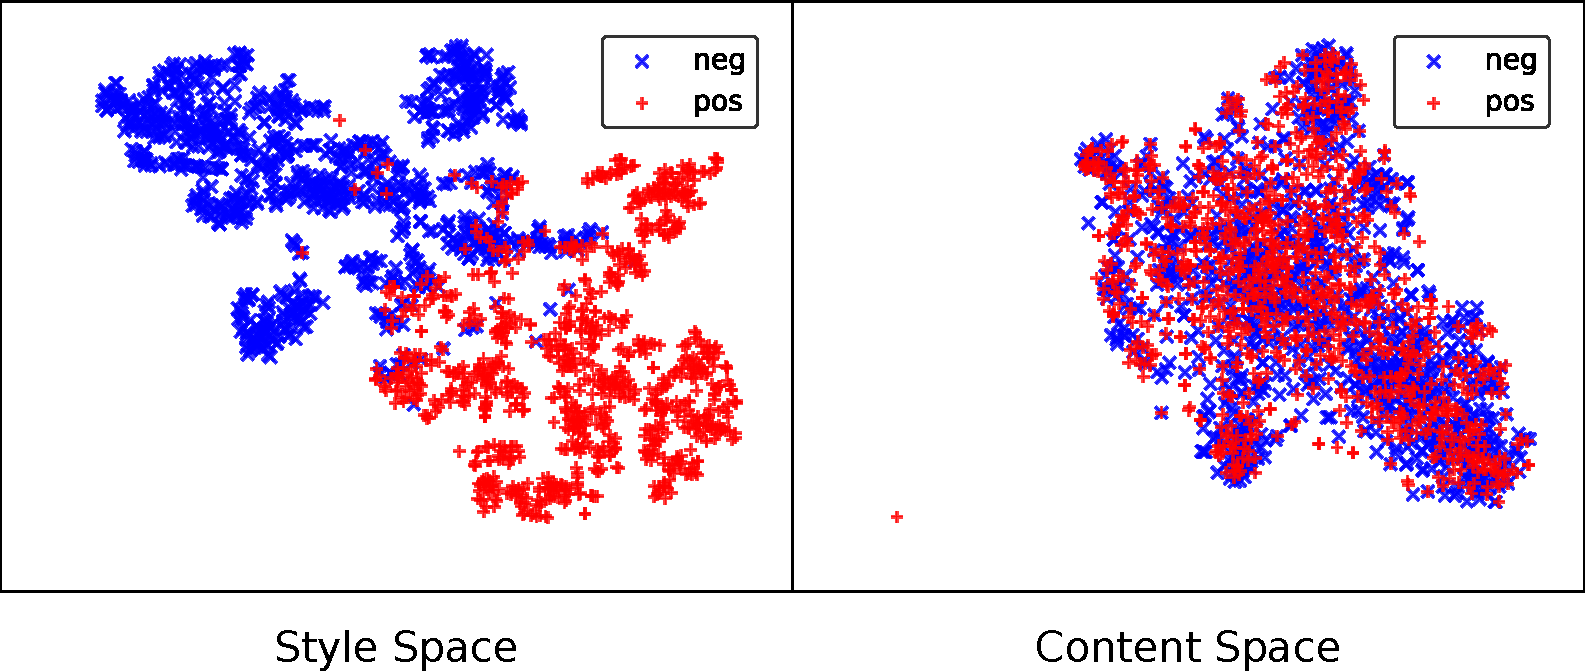
\includegraphics[width=\linewidth]{dae-latent-spaces}
	\caption{Deterministic autoencoder t-SNE plots.}
	\label{fig:dae-tsne}

	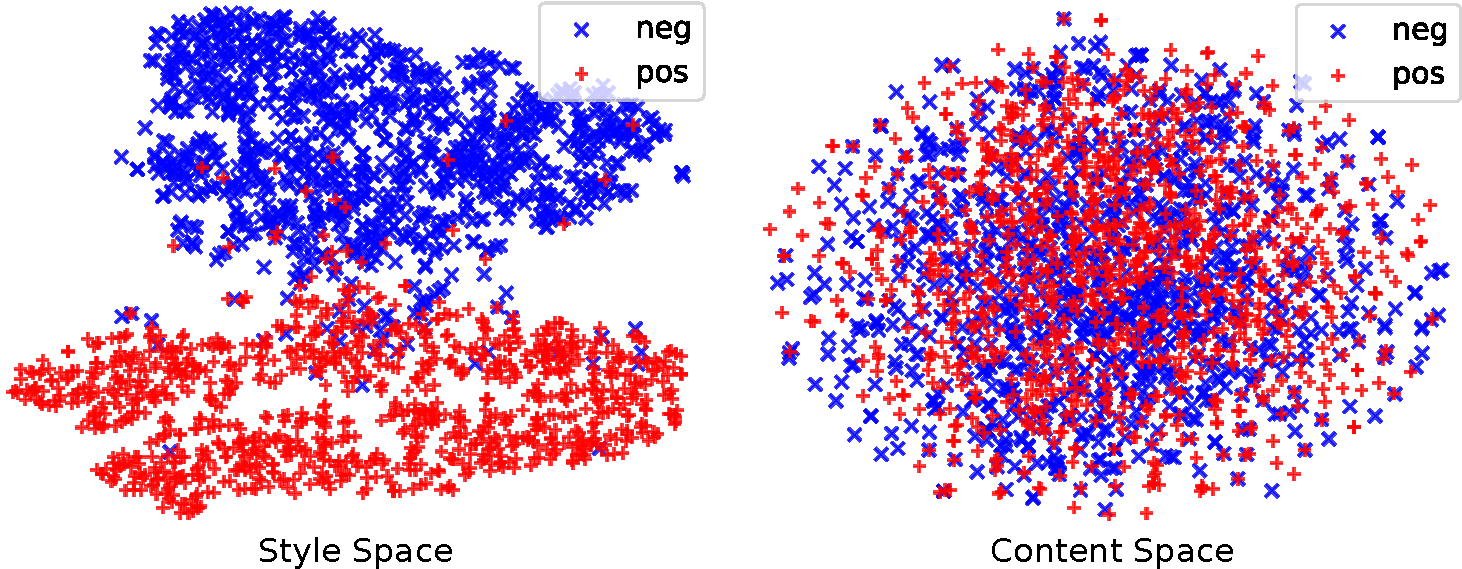
\includegraphics[width=\linewidth]{vae-latent-spaces}
	\caption{Variational autoencoder t-SNE plots.}
	\label{fig:vae-tsne}
\end{figure}

We observe that the style embedding model \cite{fu2017style} performs poorly on the style-transfer objective, resulting in inflated cosine similarity and word overlap scores.
A qualitative analysis indicates that this model resorts to simply reconstructing most of the source sentences, and is not very effective at transferring style.

Results show that, our approach achieves comparable cosine similarity and word overlap scores to previous work \cite{shen2017style,zhao2018adversarially}, and significantly better style-transfer strength scores than all of the models compared to. This indicates that our disentangled latent space can be used for better text style-transfer.
Our VAE model also produces the most fluent sentences for both tasks, which is corroborated by the manual evaluation results.

Table~\ref{tab:ablation-results} presents the results of ablation tests.
We see that both the style adversarial loss and multi-task classification loss play a role in the strength of style-transfer, and that they can be combined to further improve performance.

\begin{table}[ht]
	\centering
	\begin{tabular}{| l || c | c | c | }
		\hline
		\tabc{2}{Model}                    & \tabh{Transfer} & \tabh{Content}      & \tabh{Language} \\
		                                   & \tabh{Strength} & \tabh{Preservation} & \tabh{Quality}  \\
		\hline
		\hline
		\citeauthor{shen2017style}         &                 &                     &                 \\
		\hline
		\citeauthor{fu2017style}           &                 &                     &                 \\
		\hline
		\citeauthor{zhao2018adversarially} &                 &                     &                 \\
		\hline
		Ours (DAE)                         &                 &                     &                 \\
		\hline
		Ours (VAE)                         &                 &                     &                 \\
		\hline
	\end{tabular}
	\caption{Manual evaluation results.}
	\label{tab:manual-evaluation}
\end{table}

The manual evaluation results are presented in Table \ref{tab:manual-evaluation}.
Our VAE model attains the best score for transfer strength as well as generated sentence quality amongst all the evaluated models.

Some examples of style-transfer sentence generation are presented in Table~\ref{tab:transfer-samples}.
We see that, with the empirically estimated style vector, we can reliably control the sentiment of generated sentences.

\section{Conclusion and Future Work}
In this paper, we propose a simple yet effective approach for disentangling the latent space of neural networks using multi-task and adversarial objectives.
Our learned disentanglement approach can be applied to text style-transfer tasks.
It achieves similar content preservation scores, and significantly better style-transfer strength scores compared to previous state-of-the-art work.

For future work, we intend to evaluate the effects of disentangling the style space for datasets with greater than two distinct styles.
We would also like to explore the possibility of aligning each encoded style distribution to a unique prior, which could be sampled from at inference time for style-transfer, as opposed to using the empirical mean of training-time style embeddings.

%\section{Acknowledgements}
%We acknowledge the support of the Natural Sciences and Engineering Research Council of Canada (NSERC) [261439-2013-RGPIN], and Amazon Research Award.
%The Titan Xp GPU used for this research was donated by the NVIDIA Corporation.

\bibliography{main}
\bibliographystyle{aaai}

% \pagebreak

% \appendix

% \section{Appendix}

% \subsection{Ablation Test t-SNE plots}

% \begin{figure}[h]
% 	\captionsetup{justification=centering}
% 	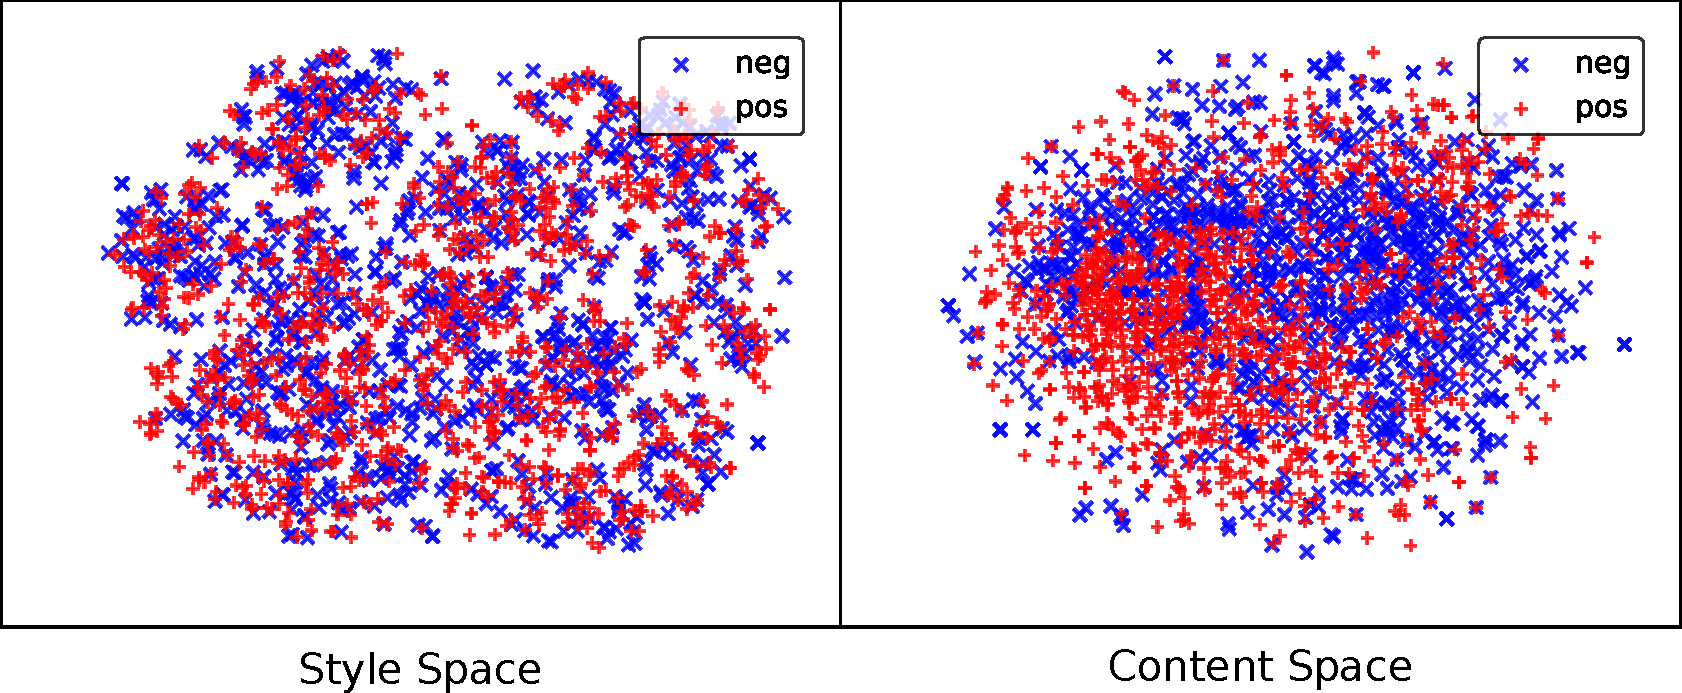
\includegraphics[width=\linewidth]{vae-latent-spaces-only-rec}
% 	\caption{t-SNE Plots: VAE with only $\loss{AE}$}
% 	\label{fig:vae-tsne-only-rec}
% \end{figure}

% \begin{figure}[h]
% 	\captionsetup{justification=centering}
% 	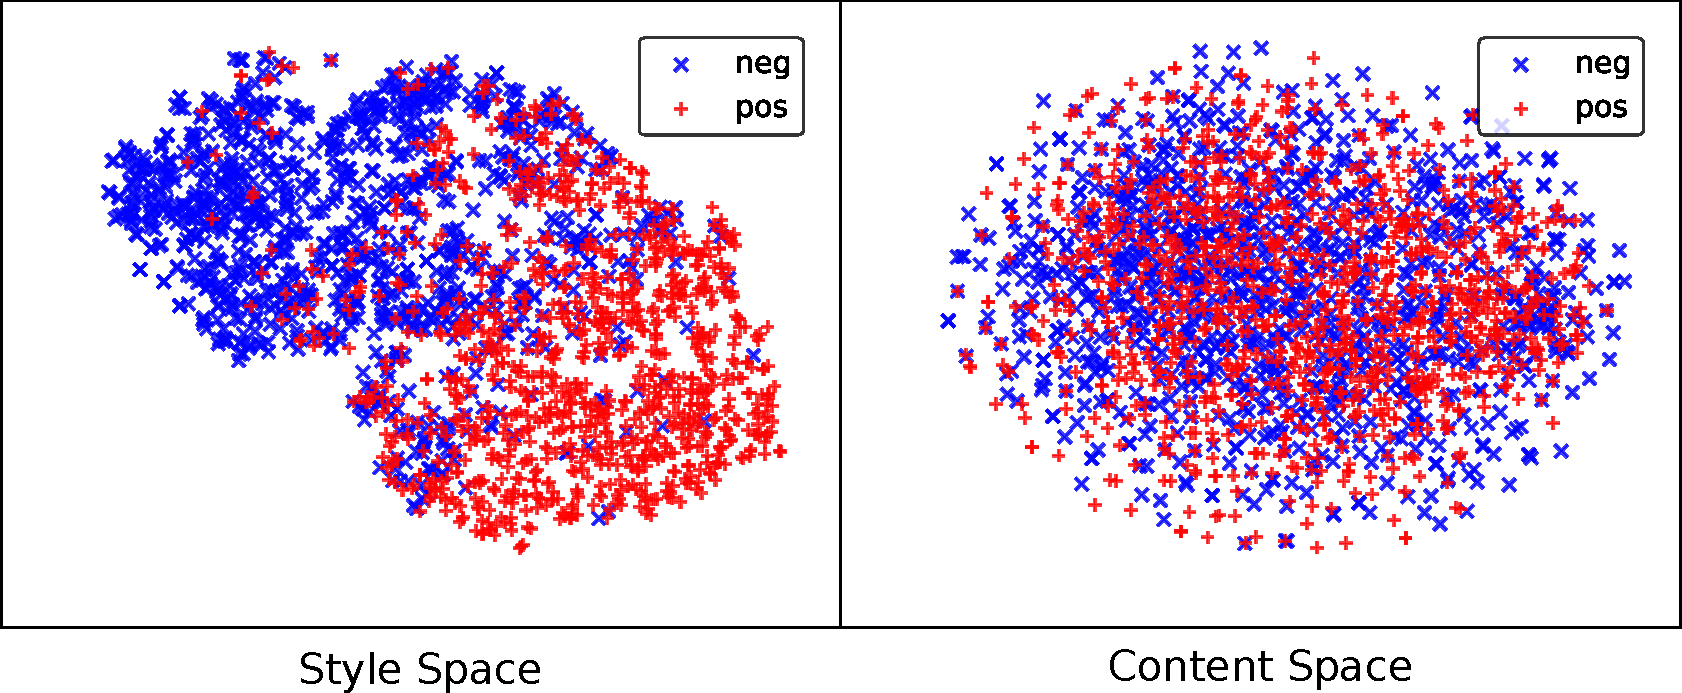
\includegraphics[width=\linewidth]{vae-latent-spaces-rec-adv}
% 	\caption{t-SNE Plots: VAE with $\loss{AE} + \loss{adv(s)}$}
% 	\label{fig:vae-tsne-rec-adv}
% \end{figure}

% \begin{figure}[h]
% 	\captionsetup{justification=centering}
% 	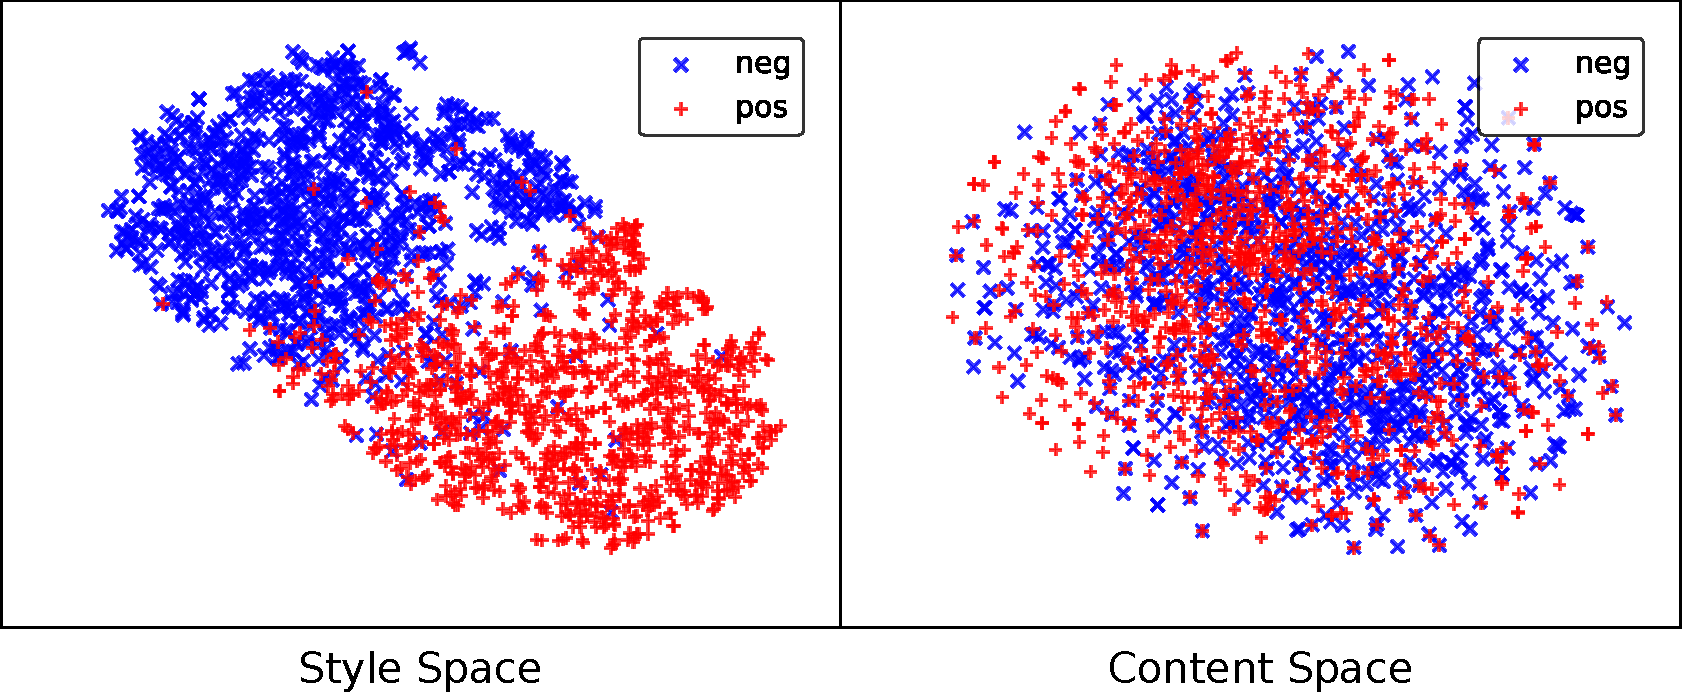
\includegraphics[width=\linewidth]{vae-latent-spaces-rec-mult}
% 	\caption{t-SNE Plots: VAE with $\loss{AE} + \loss{mul(s)}$}
% 	\label{fig:vae-tsne-rec-mult}
% \end{figure}

\end{document}
